%
% classification.tex
% 
% (c) 2019 Prof Dr Andreas Mueller
%
\chapter{Terminology and Notation
\label{chapter:terminology and notation}}
\lhead{Terminology and notation}
Partial differential equations are equations for an unknown function of
several variables, linking values of the function to its partial
derivatives.
In this chapter, we write the unknown function always as $u(x_1,\dots,x_n)$
and the independent variables as $x_1,\dots,x_n$.
\[
u\colon \mathbb R^n\to\mathbb R:(x_1,\dots,x_n)\mapsto u(x_1,\dots,x_n).
\]
We will abbreviate points of the domain of definition of such a function
as $x=(x_1,\dots,x_n)$.
We have to clarify the following aspects:
\begin{compactenum}
\item What is a partial differential equation exactly?
\item Where is it defined?
\item How do we formulate boundary conditions and initial conditions?
\item What types of partial equations are there?
\end{compactenum}

%
% equations.tex
%
% (c) 2019 Prof Dr Andreas Mueller
%
\rhead{Differential equations}
\section{Differential equations\label{klassifikation:differentialgleichungen}}
A partial differntial equation links values 
$u(x_1,\dots,x_n)$
to the values of partial derivatives
\begin{equation}
\frac{\partial u}{\partial x_1},
\frac{\partial u}{\partial x_2},
\dots,
\frac{\partial u}{\partial x_n},
\frac{\partial^2 u}{\partial x_1^2},
\frac{\partial^2 u}{\partial x_1\partial x_2},\dots,
\frac{\partial^2 u}{\partial x_1\partial x_n},\dots,
\frac{\partial^2 u}{\partial x_n^2},
\frac{\partial^3 u}{\partial x_1^3},\dots,
\frac{\partial^3 u}{\partial x_{i_1}\partial x_{i_2}\partial x_{i_3}},\dots
\label{ableitungen}
\end{equation}
In the case of a single independent variable, there is only a single
derivative of each order.
For $n$ independent variables, the number of derivatives of order $k$
increases to $n^k$.

We have a partial differential equation as soon as we know how to
link the various derivatives.
In the example of the wave equation of the form
\begin{equation}
\frac{\partial^2 u}{\partial x_1^2}
-
c^2\frac{\partial^2 u}{\partial x_2^2},
\label{wellengleichung-tform}
\end{equation}
we have combine the second derivatives 
\[
\frac{\partial^2 u}{\partial x_1^2}
\qquad
\text{und}
\qquad
\frac{\partial^2 u}{\partial x_2^2}
\]
linearly, all the other derivatives in the list
\eqref{ableitungen}
are not used.
If we write
\[
F(t_{11}, t_{22}) = t_{11} -c^2t_{22},
\]
then the wave equation
\eqref{wellengleichung-tform}
gets the form
\[
F\biggl(
\frac{\partial^2 u}{\partial x_1^2},
\frac{\partial^2 u}{\partial x_2^2}
\biggr)=0.
\]
Here we have a function $F$ that completely specifies how the
derivatives have to be combined to give the differential equation.

The function $F$ could, however, be much more involved.
E.~g.~it could also depend on the independent variables
$x_1,\dots,x_n$, the values $u(x_1,\dots,x_n)$ of the function
or on other derivatives.
And the dependence could be more complicated than just linear as
in this example.

More generally, a partial differential equation is tiven by a function
\[
F(x_1,\dots,x_n,u,\dots\text{variables for partial derivatives of $u$}\dots).
\]
The differential equation is obtained by substituting the unknown function $u$
and the partial derivatives into $F$ and setting it equal to $0$:
\[
F\biggl(x_1,\dots,x_n,u(x_1,\dots,x_n),\dots,
\frac{\partial^k u}{\partial x_{i_1}\partial x_{i_2}\dots \partial x_{i_k}},\dots\biggr)=0.
\]
A often used convention for the variables is to name the variables that
stand for first derivatives as $p_i$ and variables that stand for second
derivatives as $t_{ij}$.

\subsection{Order\label{klassifikation:ordnung}}
\index{Order}
As for ordinary differential equations, the order is the order of the
highest derivative that appears in the differential equation.

\subsubsection{Partial differential equations of first order}
In a partial differential equation of first order, only the first derivatives
show up.
It can therefore ge written in the form
\[
F\biggl(x_1,\dots,x_n, u, \frac{\partial u}{\partial x_1},\dots,\frac{\partial u}{\partial x_n}\biggr)=0.
\]
A partial differential equation of first order becomes equivalent to
a function
$F(x_1,\dots,x_n,u,p_1,\dots,p_n),$
where the substitution
\[
p_i\to \frac{\partial u}{\partial x_i}
\]
is applied.

For partial differential equations of first order with to variables,
we usually write
$F(x,y,u,p,q)$,
with the substitutions
\[
p\to\frac{\partial u}{\partial x},
\qquad
q\to\frac{\partial u}{\partial y}.
\]

\subsubsection{Partial differential equations of second order}
In the first chapter we have seen that partial differential equations of
first order are of prime importance.
Such a partial differential equation contains first and second derivatives.
Since the solution function must be differentiable, the second derivatives
do not depend on the order in which the are executed, i.~e.
\[
\frac{\partial^2 u}{\partial x_i\partial x_j}
=
\frac{\partial^2 u}{\partial x_j\partial x_i}
\quad\forall i,j
\]
The differential equation can be written as
\[
F\biggl(x_1,\dots,x_n,u,
\frac{\partial u}{\partial x_1},\dots,\frac{\partial u}{\partial x_n},
\frac{\partial^2 u}{\partial x_1^2},\dots,\frac{\partial^2 u}{\partial x_n^2}\biggr)
\]
with the function
\[
F(x_1,\dots,x_n,u,p_1,\dots,p_n,t_{11},t_{12},\dots,t_{n,n-1},t_{nn})
\]
in the variables $x_i$, $u$, $p_i$ and $t_{ij}$.
The substitution
\[
p_i\to \frac{\partial u}{\partial x_i}
,\quad
t_{ij}\to \frac{\partial^2 u}{\partial x_i\partial x_j}
\]
turns the Function $F$ into the differential equation.

The examples of partial differential equations discussed in chapter~1
correspond to the following functions:
\begin{align*}
F(t_{11},\dots,t_{nn})&=t_{11}-a^2(t_{22}+\dots+t_{nn})&&\text{wave equation}
\\
F(p_1,t_{22},\dots,t_{nn})&=p_1-a^2(t_{22}+\dots+t_{nn})&&\text{heat equation}
\\
F(t_{11},\dots,t_{nn})&=t_{11}+\dots+t_{nn}&&\text{Poisson problem}
\end{align*}

\subsection{*Multiindices and higher partial derivatives
\label{klassifikation:multiindizes}}
In the previous section we required mixed partial derivatives.
The usual notation
\[
\frac{\partial^k u}{\partial x_{i_1}\partial x_{i_2}\dots\partial x_{i_k}}
\]
quickly becomes cumbersome.
The only information needed is the numbers of the variables with respect
to which the derivative is taken, not even the order is necessary.
The notation of multiindices that we summarize in this section takes
this into account.
\begin{definition}
We call
${\bf k}=(k_1,\dots,k_n)$ a multiindex of length $n$.
The degree of this multiindex is $|{\bf k}|=k_1+\dots+k_n$.
\end{definition}
With this notation, we can write terms that often appear in multivariate
analysis much more compactly:
\begin{align*}
x^{\mathbf k}&=x_1^{k_1}x_2^{k_2}\dots x_n^{k_n}\\
\partial_{\mathbf k}u
&=\frac{\partial^{k_1}}{\partial x_1^{k_1}}\dots
\frac{\partial^{k_n}}{\partial x_n^{k_n}}u
=\frac{\partial^{|{\mathbf k}|}}{\partial x_1^{k_1}\dots\partial x_n^{k_n}}u
=D^{\mathbf k}u=D_1^{k_1}D_2^{k_2}\dots D_n^{k_n}u
\end{align*}
Of course we can use multiindices also in other contexts.
As an example, a multivariate power series can be written as
\[
f(x_1,\dots,x_n)=\sum_{\mathbf k}a_{\mathbf k}x^{\mathbf k},
\]
where $a_{\mathbf k}\in\mathbb R$ are the coefficients of the power series.

A partial differential equation of order $m$ with $n$ independent variables
no corresponds to a fucntion
\begin{align*}
F&\colon \mathbb R^n\times \mathbb R^{\{{\mathbf k}|\,|{\mathbf k}|\le m\}} \to \mathbb R
\\
&\colon(x_1,\dots,x_n,u, \dots)\mapsto F(x_1,\dots,x_n,u,\dots)
\end{align*}
The function has arguments $x_1,\dots,x_n$, $u$ and an argument for
each multiindex of degree $\le m$.
The smallest multiindex is
$(0,\dots,0)$, it corresponds to the function $u$.
For the argument with
multiindex ${\mathbf k}$ we must substitute the derivative with
this same multiindex.
Die first multiindices are
\[
(1,0,\dots,0), (0,1,\dots,0),\dots, (0,\dots, 0,1),
\]
the corresponding derivatives are the first partial derivatives:
\[
F(x_1,\dots,x_n,u,\partial_1 u,\dots,\partial_2 u,\dots)=0.
\]

\subsection{Conversion to lower order\label{klassifikation:umwandlung}}
As with ordinary differential equations, partial differential equations
of order $>1$ can be convert to a system of partial differential equations
of lower order.
We quickly recall the procedure for ordinary differential equations
and then explain what changes for partial differential equations.

The ordinary differential equation
\[
F(x,y,y',y'',\dots,y^{(n)})=0
\]
can be reduced by introducing additional functions 
$y_0,\dots,y_{n-1}$
that satisfy the equations
\begin{equation}
\begin{aligned}
\frac{dy_0}{dx}&=y_1\\
\frac{dy_1}{dx}&=y_2\\
&\vdots\\
\frac{dy_{n-2}}{dx}&=y_{n-1}\\
F\biggl(x,y_0,y_1,y_2,\dots,\frac{dy_{n-1}}{dx}\biggr)&=0
\end{aligned}
\label{classification:reduced}
\end{equation}
By setting $y_0=0$ we find
$y_k=y^{(k)}$ for each $k$, and by substituting that into the last
equation, we recover the original differential equation
$F(x,y,y',y'',\dots,y^{(n)})=0$.
The first order system \eqref{classification:reduced} is equivalent to the
original differential equation.

Now consider the partial differential equation of second order with
the two independent variables $x$ and $y$
\[
F\biggl(x,y,u,\frac{\partial u}{\partial x},\frac{\partial u}{\partial y},
\frac{\partial^2 u}{\partial x^2},\frac{\partial^2 u}{\partial x\partial y},
\frac{\partial^2u}{\partial y^2}\biggr)=0.
\]
Following the method for ordinary differential equations, we need new
functions that stand for the derivatives, e.~g.~$p(x,y)$ und $q(x,y)$.
We have to express that these functions are in fact partial
derivatives of the function $u$, this gives us the two new partial
differential equations
\[
p=\frac{\partial u}{\partial x},\qquad q=\frac{\partial u}{\partial y}.
\]
We can also express the second partial derivatives using these variables:
\begin{align*}
\frac{\partial^2 u}{\partial x^2}&=\frac{\partial p}{\partial x}\\
\frac{\partial^2 u}{\partial x\partial y}&=\frac{\partial p}{\partial y}=\frac{\partial q}{\partial x}\\
\frac{\partial^2 u}{\partial y^2}&=\frac{\partial q}{\partial y}
\end{align*}
Since we consider $p$ and $q$ as independent functions, and not as
derivates of the same function, it is not automatically clear that 
the mixed derivatives are the same, so we have to add the equation
\[
\frac{\partial p}{\partial y}
=
\frac{\partial q}{\partial x}.
\]
This gives us the following system of partial differential equations
of first order
\begin{align*}
F\biggl(x,y,u,p,q,\frac{\partial p}{\partial x},\frac{\partial p}{\partial y},\frac{\partial q}{\partial y}\biggr)&=0\\
p&=\frac{\partial u}{\partial x}\\
q&=\frac{\partial u}{\partial y}\\
\frac{\partial p}{\partial y}&=\frac{\partial q}{\partial x}
\end{align*}
Thus we have reduced a partial differential equations of second order
to a system of partial differential equations of first order for 
the three unknown functions $u$, $p$ and $q$.

%\subsection{*Umwandlung einer Gleichung beliebiger Ordnung\label{klassifikation:beliebigeordnung}}
%Sei jetzt eine partielle Differentialgleichung $m$-ter Ordnung
%gegeben. Sie hat die Gestalt
%\[
%F\bigl(
%x_1,\dots,x_n, u, \frac{\partial u}{\partial x_1},\dots,\frac{\partial u}{\partial x_n},\frac{\partial^2u}{\partial x_1^2},\frac{\partial^2 u}{\partial x_1\partial x_2},\dots,\frac{\partial^2u}{\partial x_n^2},\dots
%\bigr)=0
%\]
%wobei als Argumente Ableitungen mit Multiindizes ${\mathbf k}$ mit
%$|{\mathbf k}|\le m$ vorkommen. Daraus kann man jetzt ein System von
%partiellen Differentialgleichungen machen, indem man für jeden
%Multiindex $|{\mathbf k}|$ mit $|{\mathbf k}|\le m$ eine zusätzliche
%Funktion $p_{\mathbf k}$ einführen. In die Funktion können wir
%dann statt der Ableitungen von $u$ die Funktionen $p_{\mathbf k}$
%einsetzen.
%\[
%F\bigl(
%x_1,\dots,x_n, u, p_1,\dots,p_n,p_{(2,0,\dots)},p_{(1,1,\dots)},
%\dots,p_{(0,\dots,0,2)},\dots, \frac{\partial p_{\mathbf k}}{\partial x_i})
%\bigr)=0,
%\]
%wobei nur Ableitungen erster Ordnung vorkommen, also nur Ableitungsterme
%mit $|{\mathbf k}|\le m$.
%Dazu kommt aber eine ganze Menge von neuen Gleichungen,
%welche sagen, dass die die $p_{\mathbf k}$ eigentlich Ableitungen sind:
%\[
%\frac{\partial}{\partial x_i}p_{\mathbf k}=p_{{\mathbf k} + (0,\dots,1,\dots,0)}\quad\forall i\;\forall{\mathbf k}(|{\mathbf k}|<m),
%\]
%wobei die $1$ an der $i$-ten Stelle steht. Dazu kommen Gleichungen
%die besagen, dass die gemischten Ableitungen vertauscht werden können.
%Sei ${\mathbf k}$ ein Multiindex, und sei ${\mathbf k}'$ ein Multiindex,
%aus dem ${\mathbf k}$ entsteht, wenn man an der Stelle $i$ eins addiert.
%Ebenso sei ${\mathbf k}''$ ein Multiindex, aus dem ${\mathbf k}$ entsteht,
%wenn man an der Stellen $j$ eins addiert. Für jede solche Konstellation
%erhält man eine zusätzliche Gleichung:
%\[
%\frac{\partial}{\partial x_i}p_{{\mathbf k}'}=\frac{\partial}{\partial x_j}p_{{\mathbf k}''},
%\]
%denn beide Terme stehen ja eigentlich für $\partial_{\mathbf k}u$.

%
% domains.tex -- 
%
% (c) 2019 Prof Dr Andreas Mueller, Hochschule Rapperswil
%
\section{Transforms with more general types of domains}
Integral transforms are useful to help partial differential equations,
but only if the transform matches the domain:
\begin{center}
\begin{tabular}{cl}
Domain&Transform\\
\hline
$[0,\infty)$&Laplace transform\\
$\mathbb R$&Fourier transform\\
$[-\pi,\pi]$&Fourier series
\end{tabular}
\end{center}
The separation method has shown how this technique can be generalized.
We illustrated the basic principle for the heat equation on a domain
$G\subset \mathbb R^n$.
The differential equation is
\[
\partial_t u(t,x)=\Delta u(t,x)
\]
for $(t,x)\in [0,\infty)\times G$ with initial conditions
\[
u(0,x)=u_0(x) \quad x\in G
\]
and boundary conditions
\[
au(t,x)+b\partial_nu(t,x)=0\quad (t,x)\in[0,\infty)\times \partial G.
\]
Chapter~\ref{chapter:separation} suggests that we can find a family
of functions
$u_k(x)$ which are eigenfunctions of the Laplace operator
\[
\Delta u_k=\lambda_k u_k
\]
and satisfy homogeneous boundary conditions.
It also turns out that these functions can be used to expand any
function on $G$ into a series
\[
u_0(x)=\sum_{k=1}^\infty a_ku_k(x).
\]
No we can immediately write down the solution to the heat equation:
\[
u(t,x)=\sum_{k=1}e^{-\lambda_kt}u_k(x)
\]
Apparently, the functions $u_k$ take over the role the functions
$e^{ikx}$ had in the Fourier theory.

Modern mathematics knows a theory of harmonic analysis on so called
Lie groups, which generalize and unify Laplace transform and Fourier
transform and which allow to handle more general domains.
As an example, expansions on $n$-dimensional spheres are possible
using so called spherical functions.


%
% conditions.tex --
%
% (c) 2019 Prof Dr Andreas Mueller
%
\section{Boundary conditions\label{klassifikation:randbedingungen}}
\rhead{Boundary conditions}
\index{boundary conditions}
As with ordinary differential equations it is not enough to 
specify the partial differential equation to determine the
solution.
This section shows how the concept of initial conditions and boundary
conditions needs to be extended for partial differential equations.

\subsection{Initial and boundary conditions for ordinary differential equations\label{klassifkation:anfangswerte-ode}}
For ordinary differential equations, we have to specify initial or boundary
conditions.
To fix the differential equation
\[
y''+p(x)y'+q(x)y=0
\]
on the interval
$[0,1]$,
we need two additional conditions, any of the following types of conditions
will do:
\begin{itemize}
\item the values $y(0)$ and $y'(0)$ (initial conditions)
\item the values $y(0)$ und $y(1)$ (boundary conditions)
\item two linear equations combining these
\begin{align*}
\alpha_0y(0)+\beta_0y'(0)&=\gamma_0\\
\alpha_1y(1)+\beta_1y'(1)&=\gamma_1.
\end{align*}
%wobei die Koeffizientenmatrix auf der linken Seite regulär sein muss.
\end{itemize}

\begin{beispiel}
\begin{figure}
\centering
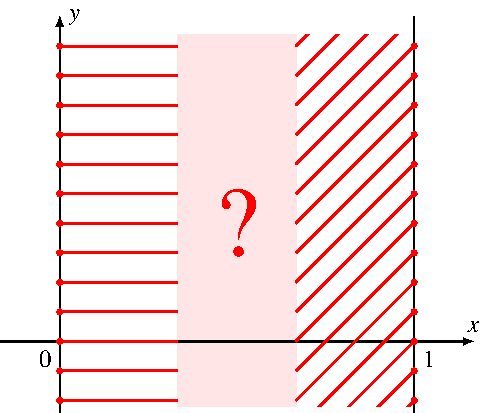
\includegraphics{2-classification/images/mismatch.pdf}
\caption{Specifying derivatives at both ends of the interval for the
differential equation $y''=0$ leads to a contradiction.
The boundary value $y'(0)=0$ means that the solution must be a straight
line with slope $0$, but the boundary value $y'(1)=1$ forces a straight
line with slope $1$.
There is no way to reconcile these conditions.
\label{boundary:mismatch}}
\end{figure}
Even for an linear ordinary differential equation of second order
not every combination of boundary values will allow a solution.
The equation
\[
y''=0
\]
means that the solution curve does not have curvature.
Consequently the solution is a straight line with equation $y=Ax+B$.
In particular, the slope must be equal at both ends of the interval.
The boundary values
\[
y'(0)=0\qquad\text{and}\qquad y'(1)=1,
\]
thus lead to a problem that has no solution (see
figure~\eqref{boundary:mismatch}).
\end{beispiel}

\subsection{Boundary values for partial differential equations\label{klassifikation:randwerte-pde}}
Specifying the boundary values for partial differential equations
becomes much more complicated.
To develop some intuition for this task, let's look again at the
vibrating string.
\begin{figure}
\begin{center}
%\includegraphics{../common/images/randwerte-1.pdf}
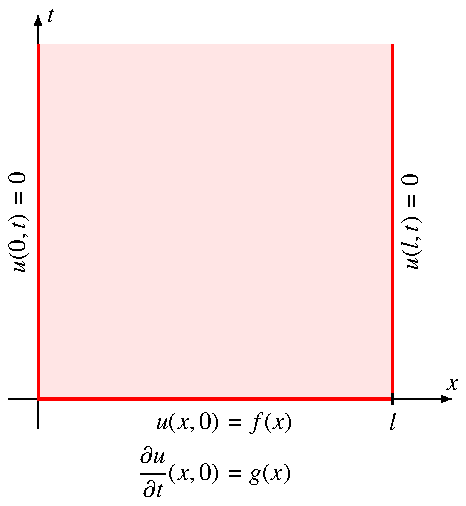
\includegraphics{2-classification/images/wave.pdf}
\end{center}
\caption{boundary values for the wave equation for a vibrating string.
The domain is colored light red, the boundary is red, the boundary
values are specified along the boundary.
\label{klassifikation:randwertesaite}}
\end{figure}
In figure \ref{klassifikation:randwertesaite}
we have drawn the domain in light red.
Boundary values can be given on the left, right and bottom portions
of the boundary.

The theory of ordinary differential equations teaches that a 
differential equation of second order needs precisly two independent
boundary values.
We can either give values at each end of an interval or the value and the
first derivative at one end.

We do the same for the wave equation.
If we forget the $t$ dependence for a moment, we are reduced to a
differential equation of second order in $x$ on the interval $[0,l]$,
so we expect that we can give boundary values at each end
as in
\[
u(0,t)=0\qquad u(l,t)=0.
\]
If we disregard the $x$-dependence, we are left with a differential equation
in $t$ for $t>0$, i.~e.~the only choice for boundary conditions is to
specify the value and the first derivative at $t=0$.

In principle there are multiple first derivatives.
However, if we already know the values of $u(x,0)=f(x)$ along the bottom
boundary, we
also know the values of the first derivative with respect to $x$, it is
\[
\frac{\partial }{\partial x}u(x,0) = f'(x)
\]
We no longer have the option to specify this derivative.
So the only derivative we can reasonably specify on the boundary
is the one with respect to $t$, or in the direction
orthogonal to the boundary.

It turns out that these boundary conditions do in fact uniquely
determine the solution.
Unfortunately this relatively straight forward discussion becomes
much more complicated for general domains.

\subsubsection{General Discussion}
Right from the start we don't even know on which part of the boundary
we should try to specify boundary conditions.
In principle we can use any part of the boundary, but it may happen
that we may not be able to choose boundary values on all of the boundary
freely.
Values on some part of the boundary may already define the values on
other parts of the boundary.

In addition, we have to decide whether to involve derivatives of the
unknown function, which we have already seen cannot be specified
arbitrarily but are subject to certain restrictions, that we would like
to highlight with the following example.
Consider the half plane
\[
\Omega=\{(x,y)\in\mathbb R^2\,|\,x>0\}.
\]
Let $u$ be a function defined on $\bar\Omega$.
If the values of $u$ are given along the boundary $\partial\Omega$
then we also know the derivatives in direction tangential to the boundary:
\[
\text{
$u(0,y)$ known
}\qquad\Rightarrow\qquad
\text{$\frac{\partial u}{\partial y}$ known.}
\]
This we can only reasonably expect to specify derivatives orthogonally
to the boundary.

Consider now the general case: the function $u$ ist defined in a point 
$x=(x_1,\dots,x_k)\in\mathbb R^k$ of the boundary $\partial\Omega$.
We assume that $\partial \Omega$ has a well defined tangential plane
in $x$.
If we know the function values along the boundary, then we know all the
partial derivatives of $u$ in directions tangent to the boundary.
They are computed using the directional derivative
\[
D_{\vec v}u(x_1,\dots,x_k)=\vec v\cdot\operatorname{grad}u
\]
for vectors $\vec{v}$ in the tangent plane.
The only derivative not known yet is the derivative in the direction
orthogonal to the tangent plane.

\begin{definition}
\label{definition:normal-derivative}
Let $\vec{n}$ be the normal vector of a tangent plane of the boundary
of a domain $\Omega$, then the {\em normal derivative}
\index{normal derivative}
is the directional derivative
\[
\frac{\partial u}{\partial n}
=
\frac{\partial u}{\partial \vec{n}}
=
\vec{n}\cdot \operatorname{grad}u .
\]
in the direction of $\vec{n}$
\end{definition}

\begin{beispiel}
Let $\Omega=\{(x,y)\in\mathbb R^2\,|\,x^2+y^2<1\}$ be the unit disk.
Find the normal derivative of the function
$u(x,y)=x^3y$
in each point on the unit circle.

The outside normal in the point $(x,y)$ is
\[
\vec n=\begin{pmatrix}x\\y\end{pmatrix}
\]
\begin{figure}
\centering
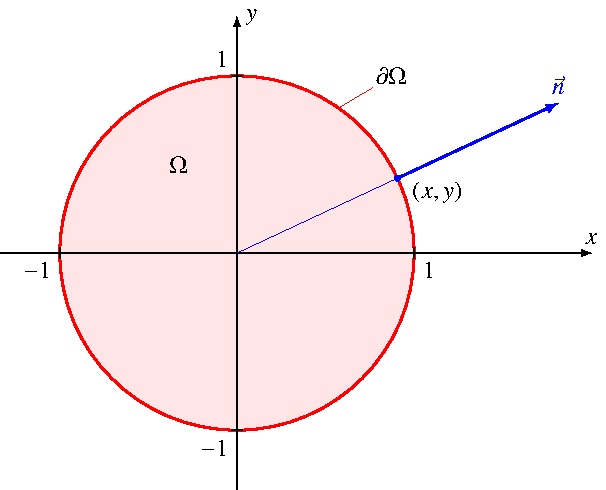
\includegraphics{2-classification/images/disk.pdf}
\caption{Outside normal of disk shaped domain
\label{conditions:outside-normal}}
\end{figure}
(see figure~\ref{conditions:outside-normal}).
The derivative of a function $u(x,y)$
in this direction then is
\[
\frac{\partial u}{\partial n}=
x\frac{\partial u}{\partial x}
+
y\frac{\partial u}{\partial y}.
\]
For the function given in the problem $u(x,y)=x^3y$:
\[
\frac{\partial u}{\partial n}
=
x\cdot 3x^2y+y\cdot x^3=
4x^3y.
\qedhere
\]
\end{beispiel}

\begin{beispiel}
\begin{figure}
\centering
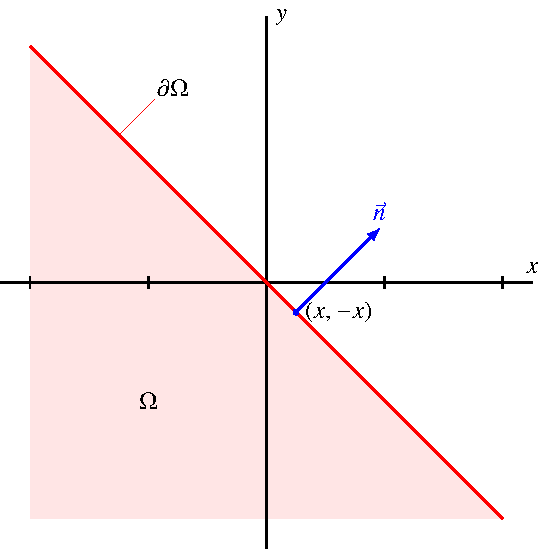
\includegraphics{2-classification/images/oblique.pdf}
\caption{Normal derivative on the boundary of the domain
$\Omega=\{(x,y)\,|\, x+y<0\}$
\label{conditions:oblique}}
\end{figure}
Find the normal derivative of the function
$x^2-y^2$
on the boundary of the domain
$\Omega=\{(x,y)\in\mathbb R^2\,|\,y+x<0\}$
(see figure~\ref{conditions:oblique}).

The domain has the straight line
$y=-x$ as boundary, which has the vector
\[
\vec n=\frac{1}{\sqrt{2}}\begin{pmatrix}1\\1\end{pmatrix}
\]
as its unit normal.
The directional derivative of $u$ in this direction 
in the point $(x,y)$ is
\[
D_{\vec n}u(x,y)
=
\vec n\cdot\operatorname{grad}u
=
\frac{1}{\sqrt{2}}
\begin{pmatrix}1\\1\end{pmatrix}\cdot\begin{pmatrix}2x\\-2y\end{pmatrix}
=
\sqrt{2}( x-y)
\]
In the point $(x,-x)$ on the boundary the normal derivative becomes
\[
\frac{\partial u}{\partial n}
=
\frac{1}{\sqrt{2}}
\frac{\partial u}{\partial x}
+
\frac{1}{\sqrt{2}}
\frac{\partial u}{\partial x}
=
\sqrt{2}(
x+x)
=
2\sqrt{2}x.
\qedhere
\]
\end{beispiel}

\subsection{Particular Cases\label{klassifikation:randwerte-speziell}}
\subsubsection{The Cauchy problem\label{klassifikation:cauchy-problem}}
\index{Cauchy problem}
The boundary of a domain usually consists of many more than just a few
points, usually of curves and surfaces.
To better understand the problem of specifying boundary conditions
we look more closely at the case of a function $u(x,y)$ of two independent
variables.
The solution function $u(x,y)$ can be visualized as a surface over the
$x$-$y$-plane also called the graph of $u$.

The boundary of a domain in $\mathbb R^2$ ist a curve.
If we prescribe values of the function $u(x,y)$ on this curve, we
essentially prescribe a curve contained in the graph of $u$.
This is called the {\em Cauchy problem}: given a curve in $\mathbb R^3$, 
find a function $u$ such that the graph of $u$ is a surface containing
the curve.

\subsubsection{Partial differential equations of first order}
An ordinary differential equation of first order only needs a single
initial value.
By analogy, we expect that should be able to solve a partial differential
equation of first order on the domain $\{x>0\}$ with only boundary values
on the $y$-axis.
Thus we expect that 
\[
u(0,y)=g(y)
\]
uniquely determines the solution.

If we assume that $g$ is continuously differentiable,
then
\[
\frac{\partial u}{\partial y}(0, y)=g'(y),
\]
the partial derivative with respect to $y$ along the $y$-axis is already
fixed.

A partial differential equation of first order defines a relation
of the form
\[
F(x,y,u(x,y), \partial_x u, \partial_y u)=0
\]
between function and partial derivatives.
For not too complicated functions $F(x,y,u,p,q)$ we can solve for
$p$, in many cases up to the boundary.
If $u(x,y)$ is a solution of the Cauchy problem, then
\begin{align*}
0&=
F(x,y,u(x,y), \partial_x u(x,y), \partial_y u(x,y)
\\
\Rightarrow
0&=
\lim_{x\to 0}
F(x,y,u(x,y), \partial_x u(x,y), \partial_y u(x,y)\\
&=F(0,y,u(x,y),\partial_x u(0,y), \partial_y u(0,y))
\\
&=
F(0,y,g(y),\underbrace{\partial_x u(0,y)}_{\displaystyle p}, g'(y)).
\end{align*}
Since we have assumed that the equation $F=0$ can be solved 
for $p$, we conclude that 
$\partial_x u(0,y)$
is already defined by the initial conditions.

The Cauchy problem for a partial differential equation of first order
only has to specify initial values along a straight line or more generally
a curve.
Boundary conditions for the derivatives are not necessary, as they can
be obtained from the differential equation.

Instead of specifying the values along the $y$-axis, we could give values
in a point on the boundary the derivative in a direction tangential to
the boundary all the way along the boundary.
To fix ideas, assume that point is $(0,0)$ and the direction of the
boundary is the $y$-axis.
Then we would give 
\begin{align*}
u(0,0)&=u_0\\
\frac{\partial u}{\partial y}(0,y)&=h(y).
\end{align*}
This does not lead to a new type problem, because by integrating
the ordinary differential equation
\[
g'(y)=\frac{\partial u}{\partial y}(0,y)=h(y)
\]
for the unknown function $g(y)$ with initial condition $g(0)=u_0$
we can recover the initial values $g(y)$.
This again confirms that for this type of equation specifying 
initial values along a section of the boundary is the basic problem
that we need to be able to solve.

\subsubsection{Partial differential equations of second order}
For an ordinary differential equation of second order we need to specify
to items as initial conditions.
Typically these will be an initial value and an initial first derivative.

For a {\em partial differential equation} of second order we thus expect 
similarly the we will have to specify first order derivatives on the
boundary in addition to boundary values.
As we have shown in the preceding sections, the first order derivatives
along the boundary are already known as soon as the boundary values are
fixed.
So boundary conditions can really only specify derivatives in the direction
normal to the boundary.
We therefore have the following two types of boundary conditions:
\begin{align}
&\text{Dirichlet boundary conditions:}&
u(0,y)&=g(y)&
\label{klassifikation:dirichlet-randbedingung}
\\
&\text{Neumann boundary conditions:}&
\frac{\partial u}{\partial x}(0,y)&=h(y)
\label{klassifikation:neumann-randbedingung}
\end{align}
\index{Dirichlet boundary conditions}
\index{boundary conditions!Dirichlet}
\index{Neumann boundary conditions}
\index{boundary conditions!Neumann}

\subsubsection{Arbitrary initial curve}
\begin{figure}
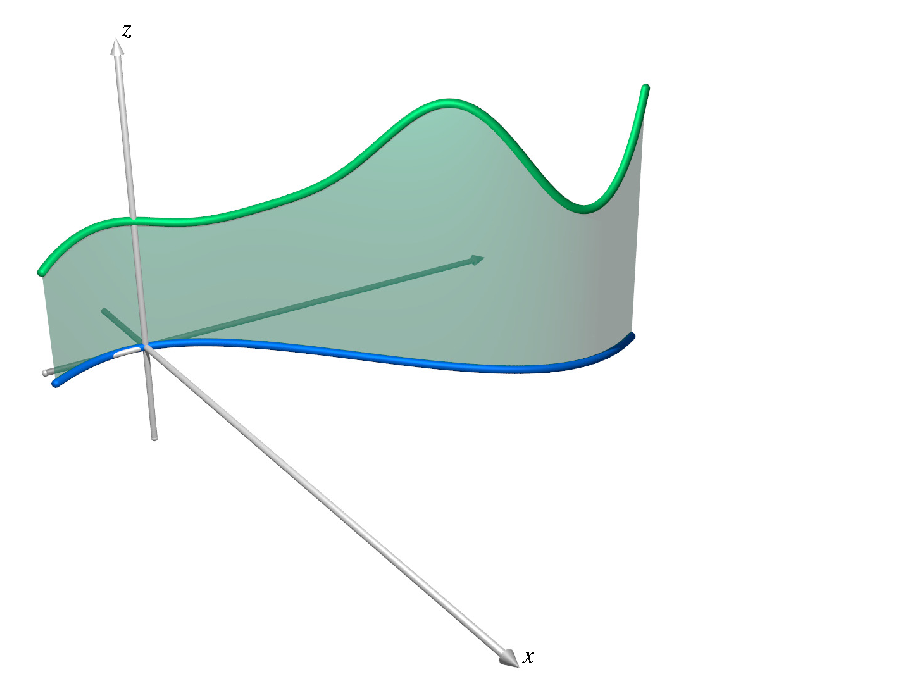
\includegraphics{2-classification/images/cauchycurve.pdf}
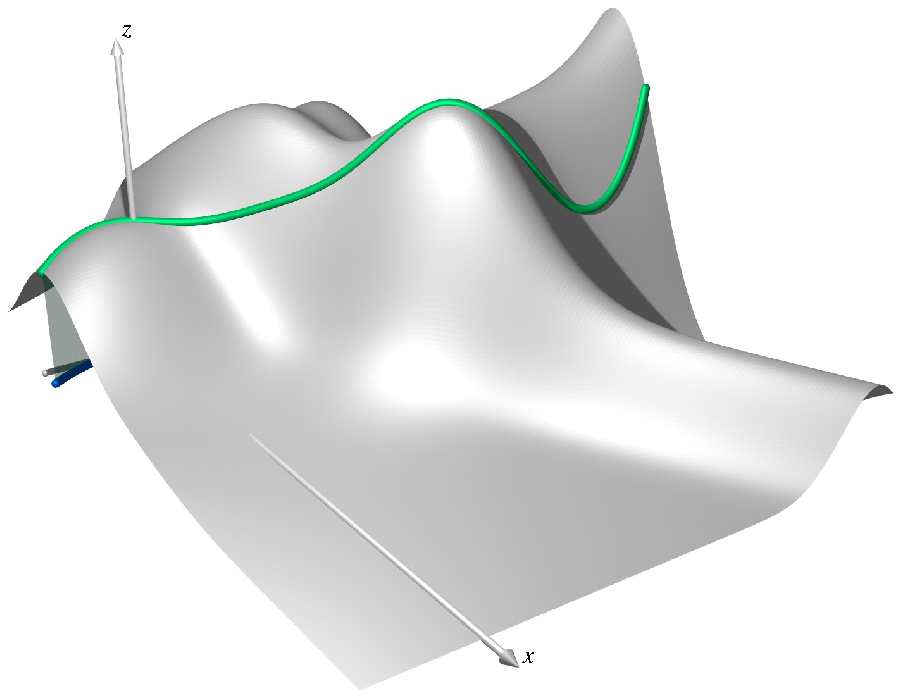
\includegraphics{2-classification/images/cauchy.pdf}%
\caption{Initial curve (top) and surface through the curve (bottom)
\label{cauchy:curve}}
\end{figure}
In general the boundary of a domain is more complicated than just 
a coordinate axis.
Fixing values along the $y$-axis means requesting that the solution
surface contains a curve that projects to the $y$ axis.
A parametrization of the curve would be $y\mapsto (0,y,g(y))$.

The generalization of this idea is the Cauchy problem:

\begin{problem}[Cauchy Problem]
Let $\gamma$ bi a curve in space and 
$F(x,y,u,\partial_xu,\partial_yu)=0$ a partial differential equation.
A function $u(x,y)$ is a solution of the Cauchy problem with initial
curve $\gamma$ if the graph of $u$ contains $\gamma$.
\end{problem}

For each point on the boundary, we can choose a coordinate system such
that the $y$-direction is tangential to the boundary while the $x$-axis
is normal on the boundary.
Then the derivatives we may specify in addition to the boundary
values is just the derivative with respect to $x$.
This derivative is just a directional derivative in a direction normal
to the boundary, we write it
\[
\frac{\partial u}{\partial n}
\]
and call it the normal derivative.
With the choice of coordinate system as describe above, the normal
derivative can be computed using the formula
\[
\frac{\partial u}{\partial n}
=\frac{\partial u}{\partial x}.
\]

If $n$ is the normal vector of a curve ($n=2$) or a surface ($n=3$),
on which boundary conditions are prescribed, then the normal derivative
can be computed using the directional derivative:
\[
\frac{\partial u}{\partial n}=D_nu = n\cdot \operatorname{grad} u.
\]
(See definition~\ref{definition:normal-derivative})

\subsection{General boundary value problem
\label{klassifikation:allgemeines-randwertproblem}}
For partial differential equations the topology of the domain has much
greater influence on the solvability than with ordinary differential
equations, where the topology of the domain is exceedingly simple.
The Cauchy problem discussed in the preceding sections helps us understand
what types of boundary conditions are meaningful.
We have seen that in general, boundary conditions are of the following types:
\begin{itemize}
\item
Values along the boundary of the domain in the form
\[
u(x)=g(x)\quad \forall x\in\partial G\subset \mathbb R^n.
\]
These are called {\em Dirichlet} boundary conditions.
\item
Values of the normal derivative along the boundary, written as
\[
\frac{\partial u}{\partial n}(x)=h(x)\quad\forall x\in\partial G\subset \mathbb R^n.
\]
These are {\em Neumann} boundary conditions.
\item
Linear combinations of values and normal derivatives along the 
bounary.
\end{itemize}
A nice example for mixed boundary conditions is the wave equation of
a vibrating string.
For $t=0$ we specify initial values and initial $t$-derivatives which happen
to be normal derivatives.
These normal derivatives are not needed on the two ends of the interval
for $t>0$.
So we find two types boundary conditions: boundary values along the complete
boundary and normal derivatives times the characteristic function of
the bottom boundary.

Unfortunately, this is not enough to decide which boundary conditions are needed
to fix the solution of the equation.
For this a more in depth theory is required.
This is in stark contrast to the situation for ordinary differential
equations where the Picard-Iteration method guarantees existence and
uniqueness of solutions under very mild conditions on the differential
equation.
We tackle this difficult problem for different types of differential
equations in the following chapters.
But first we must define what it means to have a solution of a partial
differential equation.

%
% solutions.tex
%
% (c) 2019 Prof Dr Andreas Mueller
%
\section{Solutions of partial differential equations\label{klassifikation:loesung}}
To solve a partial differential equation, the following data has to be
specified:
\begin{enumerate}
\item
A differential equation, e.~g.~by specifying the function $F$
\item
A domain $\Omega$
\item
Boundary values on part of the boundary $\partial\Omega$.
\end{enumerate}
\begin{definition}
A solution of a partial differential equation is a function $u$
defined on $\bar \Omega$ (not only on $\Omega$!), which is
differentiable in $\Omega$, satisfies the differential equation in
$\Omega$, and satisfies the boundary conditions on $\partial\Omega$.
\end{definition}

A problem is called {\em well posed} if the data determines the solution
uniquely.
The theory to be developed in subsequent chapters has to be able to
determine whether a problem is well posed.
Only then does it make sense to try to use a numerical algorithm
and to expect a well behaved solution.


%
% types.tex
%
% (c) 2008 Prof Dr Andreas Mueller
%
\section{Spezielle Typen von partiellen Differentialgleichungen\label{klassifikation:spezielletypen}}
\rhead{Spezielle PDGL}
Für einige spezielle Typen von Differentialgleichungen werden wir
die Frage nach Existenz und Eindeutigkeit einer Lösung beantworten
können, und manchmal sogar eine explizite Lösung angeben können.
Dazu gehören die linearen und die quasilinearen partiellen
Differentialgleichungen, die in diesem Abschnitt beschrieben werden.

\subsection{Lineare partielle Differentialgleichungen\label{klassifikation:linear}}
Die bisher vorgestellten Differentialgleichungen sind also alle lineare
Ausdrücke in den ersten und zweiten Ableitungen, man könnte sie in der
Form
\begin{align*}
\sum_{i,j=1}^n a_{ij}(x)\frac{\partial}{\partial x_i} \frac{\partial}{\partial x_j}\psi(x)
+\sum_{i=1}^na_i(x)\frac{\partial}{\partial x_i}\psi(x)&=f(x)
\\
\sum_{i,j=1}^n a_{ij}(x)\partial_i \partial_j\psi(x)
+\sum_{i=1}^na_i(x)\partial_i\psi(x)&=f(x)
\end{align*}
Die Gleichung heisst homogen, wenn $f=0$ ist.

Damit diese Probleme überhaupt eine Lösung haben, müssen noch 
Randbedingungen hinzugefügt werden.
Auch diese lassen sich in der Form linearer Gleichungen zwischen den 
Funktionswerten und den Normalableitungen von $\psi$ auf dem Rand des
Gebietes gegeben:
\begin{align*}
a\psi(x)+
b\frac{\partial}{\partial n}\psi(x)
&=g(x)\quad\forall x\in\gamma\\
a\psi(x)+b\partial_n\psi(x)&=g(x)\quad\forall x\in\gamma
\end{align*}
Die Randbedingungen heissen homogen, wenn $g=0$ ist.

Sind $\psi_1$ und $\psi_2$ zwei Lösungen der homogenen Gleichungen und der
homogenen Randbedingungen, dann ist auch $\alpha_1\psi_1+\alpha_2\psi_2$
Lösungen der homogenen Gleichung under homogenen Randbedingungen:
\begin{align*}
&\sum_{i,j=1}^n a_{ij}(x)\partial_i \partial_j
(\alpha_1\psi_1(x)+\alpha_2\psi_2(x))
+\sum_{i=1}^na_i(x)\partial_i
(\alpha_1\psi_1(x)+\alpha_2\psi_2(x))
\\
+
\alpha_1
&\sum_{i,j=1}^n a_{ij}(x)\partial_i \partial_j
\psi_1(x)
+
\alpha_1
\sum_{i=1}^na_i(x)\partial_i
\psi_1(x)
\\
+
\alpha_2
&\sum_{i,j=1}^n a_{ij}(x)\partial_i \partial_j
\psi_2(x)
+
\alpha_2
\sum_{i=1}^na_i(x)\partial_i
\psi_2(x)
=0
\end{align*}
oder für die Randbedingung
\begin{align*}
a(\alpha_1\psi_1(x) +\alpha_2\psi_2(x))
\;+&b\partial_n
(\alpha_1\psi_1(x) +\alpha_2\psi_2(x))\\
=\alpha_1(a\psi_1(x)
\;+&b\partial_n
\psi_1(x))\\
+\;\alpha_2(a\psi_2(x)
\;+&b\partial_n
\psi_2(x))
=0\quad\forall x\in\gamma
\end{align*}
Die Lösungen einer homogenen partiellen Differentialgleichung
bilden also einen Vektorraum. Insbesondere lassen sich beliebige
Lösungen der inhomogenen Differentialgleichung dadurch finden, dass
man eine partikuläre Lösung $\psi_p$ der homogenen Differentialgleichung
findet, und dazu eine beliebige Lösung der homogenen Differentialgleichung
$\psi_h$ hinzuaddiert.

\subsection{Quasilineare partielle Differentialgleichungen erster Ordnung\label{klassifikation:quasilinear}}
Einen interessanten Spezialfall bilden die quasilinearen PDGL erster
Ordnung. Sie sind nicht unbedingt linear, aber die partiellen
Ableitungen erster Ordnung kommen nur linear vor. Die Funktion
$
F(x,y,u,p,q)
$
ist also linear in $p$ und $q$. Die Variablen $x$ und $y$ sowie die
gesuchte Funktion können daher nur in den Koeffizienten der
Variablen $p$ und $q$ vorkommen, $F$ muss von der Form
\[
F(x,y,u,p,q)=a(x,y,u)p+b(x,y,u)q+c(x,y,u)
\]
sein. Eine quasilineare Differentialgleichung in zwei Variablen
hat also die Form
\[
a(x,y,u(x,y))\frac{\partial u}{\partial x}+b(x,y,u(x,y))\frac{\partial u}{\partial y}
=c(x,y,u(x,y)).
\]
Für mehr Variablen $x_1,\dots,x_n$ gilt analog, dass eine quasilineare
Differentialgleichung die Form
\[
a_1(x_1,\dots,x_n,u)\frac{\partial u}{\partial x_1}
+
a_2(x_1,\dots,x_n,u)\frac{\partial u}{\partial x_2}
+\dots
+
a_n(x_1,\dots,x_n,u)\frac{\partial u}{\partial x_n}
=c(x_1,\dots,x_n,u)
\]
hat.

Natürlich lassen sich auch quasilineare partielle Differentialgleichungen
höherer Ordnung definieren, in einer solchen Differentialgleichung
kommen zwar höheren partielle Ableitungen vor, aber immer nur linear,
man kann sie also immer in der Form schreiben:
\[
\sum_{\bf k} a_{\bf k}(x,y,u)\partial_{\bf k} u(x,y) = 0,
\]
worin die Funktionen $a_{\bf k}(x,y,u)$ nur für endlich viele
Multiindizes ${\bf k}$ von $0$ verschieden sind.

\subsection{Nichtlineare Gleichungen\label{klassifikation:nichtlinear}}
Die bisher vorgestellten Beispiele von partiellen Differentialgleichungen
sind alle linear. Viele Gleichungen der Physik sind jedoch
nicht linear.  Berühmtestes Beispiel sind die Gleichungen, die
die Strömung eines Gases beschreiben. Bereits Leonhard Euler hat 
für die Strömung eines idealen Gases ein System von partiellen
\index{Dichte}
\index{Druck}
Differentialgleichungen gefunden für die Dichte $\varrho$, den Druck
$p$ und die Strömungsgeschwindigkeit $\vec v$, alle drei sind Funktionen
\index{Stromungsgeschwindigkeit@Str\ömungsgeschwindigkeit}
von allen drei Raumkoordinaten und der Zeit. Die wichtigste davon
ist die Eulersche Gleichung:
\index{Eulersche Gleichung}
\begin{align*}
\frac{\partial \vec v}{\partial t}
+(\vec v\cdot \nabla)\vec v
=-\frac1{\varrho}\operatorname{grad}p
\\
\frac{\partial v_i}{\partial t}
+\sum_{j=1}^3v_j\frac{\partial v_i}{\partial x_j}
=
-\frac1{\varrho}\frac{\partial p}{\partial x_i}
\end{align*}
Diese Gleichung kann nicht linear sein, weil im zweiten Term
Produkte von $v_j$ mit Ableitungen von $v_i$ vorkommen.
Berücksichtigt man auch noch die Zähigkeit, wird die Gleichung
noch komplizierter:
\[
\varrho\left(
\frac{\partial\vec v}{\partial t}
+
(\vec v\cdot\nabla)\vec v
\right)
=
-\operatorname{grad}p+\eta\Delta \vec v+\left(\zeta+\frac{\eta}3\right)
\operatorname{grad}\operatorname{div}\vec v
\]

In einer Dimension bleibt von dieser Gleichung nur noch eine Komponente
$u(t,x)$ übrig, für die eine Gleichung der ungefähren Form
\[
\frac{\partial u}{\partial t}+u\frac{\partial u}{\partial x}
=\eta\frac{\partial^2u}{\partial x^2}
\]
gelten muss (wir haben den Druckgradienten vernachlässigt und
$\varrho = 1$ angenommen). Diese Gleichung wurde von
Johannes Martinus Burgers ausgiebig studiert, und heisst
daher Gleichung von Burgers.
Eine Lösung des Anfangswertproblems der Gleichung von Burgers kann 
in expliziter Form gefunden werden, wir beschreiben diese in Kapitel
\ref{chapter-nichtlinear}.



%
% notation.tex
% 
% (c) 2019 Prof Dr Andreas Mueller
%
\section{Appendix: Notation}
\rhead{Notation}
The traditional way to write derivatives isn't very compact, which is why
we will use the following equivalent notation
\begin{align*}
\frac{\partial f(x,y)}{\partial x}
&=\frac{\partial}{\partial x}f(x,y)
=\partial_x f(x,y)\\
\frac{\partial f}{\partial x_i}(x,y)
&=\partial_{x_i}f(x,y)=\partial_if(x,y)
\end{align*}
We will also use the following operator notation for derivatives:
\begin{align*}
\frac{\partial}{\partial x}
&=
\partial_x\\
\frac{\partial}{\partial x_i}
&=
\partial_{x_i}
=\partial_i
\end{align*}
In this notation, the well known opeators can be written as:
\begin{align*}
\Delta &=\partial_x^2+\partial_y^2+\dots=\sum_{i=0}^n\partial_i^2\\
\operatorname{grad}&=\nabla=\begin{pmatrix}\partial_1\\\vdots\\\partial_n\end{pmatrix}
\end{align*}
The normal derivative which is used in boundary conditions for partial
differential equations is written as
\[
\frac{\partial u}{\partial n}=\partial_nu.
\]



\section{Summary}
\begin{enumerate}
\item
A partial differential equation is specified by a function $F$
of the independent variables, of the function $u$ and of placeholders
for the partial derivatives of $u$.
\item
The order of a partial differential equation is the order of the
highest order partial derivative.
\item
In two dimensions, a partial differential equation of first order can
always be described by a function $F(x,y,u,p,q)$.
The variables $p$ and $q$ are place holders for the first partial
derivatives of $u$:
\[
F\biggl(
x,y, u,
\frac{\partial u}{\partial x},
\frac{\partial u}{\partial y}
\biggr)=0.
\]
\item
A partial differential equation can always be reduced to a system
of partial differential equations of first order.
(\ref{klassifikation:umwandlung}).
\item
\index{linear}
\index{partial differential equation!linear}
Linear partial differential equations are have $F$ depend on the function 
$u$ and the derivatives only linearly.
In two dimension, this means that $F(x,y,u,p,q)$ is linear in
$u$, $p$ and $q$.
\item
A {\em quasilinear} partial differential equation is linear in all
\index{quasilinear}
\index{partial differential equation!quasilinear}
partial derivatives, but not necessarily in the function $u$ itself.
(\ref{klassifikation:quasilinear}).
\item
The domain $\Omega$ where a differential equation is defined
has a significant influence on the solution
(\ref{klassifikation:gebiete}).
\item
The solution becomes well defined only after suitable boundary conditions
have been specified
(\ref{klassifikation:randbedingungen}). 
\item
For partial differential equations of first order we expect to specify
values of the function on part of the boundary (Cauchy problem).
\item
For partial differential equations of second order we expect to
specify values (Dirichlet boundary conditions)
and or normal derivatives (Neumann boundary conditions).
\item
A solution of a partial differential equation is a function defined
on the closure of the domain, that satisfies the differential equation
in the domain and boundary conditions on the boundary.
(\ref{klassifikation:loesung}).
\end{enumerate}
